%
% File acl2016.tex
%
%% Based on the style files for ACL-2015, with some improvements
%%  taken from the NAACL-2016 style
%% Based on the style files for ACL-2014, which were, in turn,
%% Based on the style files for ACL-2013, which were, in turn,
%% Based on the style files for ACL-2012, which were, in turn,
%% based on the style files for ACL-2011, which were, in turn, 
%% based on the style files for ACL-2010, which were, in turn, 
%% based on the style files for ACL-IJCNLP-2009, which were, in turn,
%% based on the style files for EACL-2009 and IJCNLP-2008...

%% Based on the style files for EACL 2006 by 
%%e.agirre@ehu.es or Sergi.Balari@uab.es
%% and that of ACL 08 by Joakim Nivre and Noah Smith

\documentclass[11pt]{article}
\usepackage{acl2016}
\usepackage{times}
\usepackage{url}
\usepackage{latexsym}
\usepackage{amsmath}
\usepackage{amssymb}
\usepackage{color,soul}
\usepackage[pdftex]{graphicx}
\usepackage{todonotes}

%\aclfinalcopy % Uncomment this line for the final submission
%\def\aclpaperid{***} %  Enter the acl Paper ID here

%\setlength\titlebox{5cm}
% You can expand the titlebox if you need extra space
% to show all the authors. Please do not make the titlebox
% smaller than 5cm (the original size); we will check this
% in the camera-ready version and ask you to change it back.

\newcommand\BibTeX{B{\sc ib}\TeX}
\newcommand\toin{\todo[inline]}

\title{Local Named Entity Disambiguation with Neural Attention}

\author{First Author \\
	Affiliation / Address line 1 \\
	Affiliation / Address line 2 \\
	Affiliation / Address line 3 \\
	{\tt email@domain} \\\And
	Second Author \\
	Affiliation / Address line 1 \\
	Affiliation / Address line 2 \\
	Affiliation / Address line 3 \\
	{\tt email@domain} \\}

\date{}

\begin{document}
\maketitle
\begin{abstract}
	Hello, My name is. what? my name is. who?
	My name is. what? my name is. who?
	My name is. what? my name is. who?
	My name is. what? my name is. who?
	My name is. what? my name is. who?
	My name is. what? my name is. who?
	My name is. what? my name is. who?
	My name is. what? my name is. who?
	My name is. what? my name is. who?
	My name is. what? my name is. who?
	My name is. what? my name is. who?
	My name is. what? my name is. who?
	My name is. what? my name is. who?
	My name is. what? my name is. who?
	My name is. what? my name is. who? Lorem ipsum.
\end{abstract}



\section{Introduction}

\toin{The intro is currently super-drafty (even after my pass). My comments are mainly intended to restructure the flow and point out our main arguments. We will refine it over and over again until we're sababa with it :)}

Named Entity Disambiguation (NED) is the task of linking mentions within a fragment of text against a given knowledge base of entities, such as Freebase or Wikipedia. It has been recognized as an important component in semantic parsing \cite{berant2013semantic}, as well as other NLP tasks.
\toin{These tasks don't really interest the NLP community these days... text categorization is considered virtually "solved", and IR is uncompetitive because Google, unlike academia, has the ability to A/B test its solutions.}
\toin{Also, if we intend to perform some extrinsic evaluation (e.g. plug our NED into a QA system), we should name that task explicitly, and even cite the particular paper we intend to augment.}
\toin{Question: are we dealing with finding the span as well, or given the span, are we just trying to link it to the right concept? The exact definition should appear here, and this distinction needs to be discussed in the background.}

NED algorithms can broadly be divided into local and global approaches. Local algorithms disambiguate each mention independently using local context (e.g. the rest of the sentence), whereas global approaches assume some coherence among mentions within a single document, and try to disambiguate all mentions simultaneously. Global algorithms have significantly outperformed the local approach on standard datasets \cite{ratinov2011local,guo2014entity,pershina2015personalized}. \todo{add newer stuff} However, most standard datasets are based on news corpora and Wikipedia, which are naturally coherent, well-structured, and rich in context. Other domains, such as web page fragments, social media, or questions, lack the sufficient coherence and context for global models to pay off.\todo{Potentially give citations for each domain.}

\toin{Question: could we create a similar dataset of questions or tweets? I think this would provide a much more versatile benchmark, and perhaps allow more cases for your method to shine.}
\toin{You start by telling the point about global vs local, and mentioning (too lightly) that current datasets favor global algorithms. Rather than delivering the punchline, you start talking about deep learning. I have restructured the intro to reflect the first point, and moved the DNN literature to the "background" section.}

In this work, we investigate the task of NED in a setting where only local context is available. In particular, we create a dataset of 17\todo{insert actual number} sentences containing 42\todo{insert actual number} mentions of named entities, extracted from web page fragments. This dataset is significantly larger than previously collected ones\todo{add cites}, allowing us to train a neural...\todo{continue from here}
\toin{This sentence, or the one/two that follows, needs to state the algorithmic innovation. By "innovation", I mean: what does it do differently from Globerson/Yamada?}
\toin{Mention this as well: "We also describe a novel method for initializing word and entity embeddings used in our model and demonstrate its importance." What is its importance?}

\toin{Incorporate the information from here into the new flow}
To test our method we craft a large-scale dataset of short web fragments containing mentions disambiguated into Wikipedia by thousands of website editors. Our dataset is extracted from a subset of the Wikilinks dataset \cite{singh12:wiki-links} which is re-purposed for NED. It represents a large-scale and difficult task with \hl{count} unique mentions disambiguated into $100K$ unique entities and where context is limited and noisy. We demonstrate our model greatly outperforms existing state-of-the-art NED algorithms on this dataset and in addition examine our algorithm on CoNLL \cite{hoffart2011robust}, a standard NED dataset, and show results comparable to other state-out-the-art methods on a smaller and cleaner dataset.

\toin{What are the main results? Conclusions? What have we learned from this paper? Why is it important that this paper is accepted?}



\section{Background}

\toin{This section provides readers who are less familiar with the literature the necessary information to understand your contribution. Things that need to appear in this section:

- Previous work on NED.

- An in-depth survey of the existing datasets and how they were built.

- Neural work on NED.

At the end of each paragraph/subsection, mention how this work improves upon / differs from what you just discussed.
}

%Deep Neural Networks (DNN) have recently gained traction as state-of-the-art architectures that can model powerful data representations and complex feature interaction. DNNs achieve state-of-the-art results on a wide variety of tasks ranging from image classification \cite{krizhevsky2012imagenet} to machine translation \cite{bahdanau2014neural}. For the task of NED, He at el. \shortcite{he2013learning} used stacked auto-encoders to learn entity and context representations. More recently Sun at el. and Francis-Landau at el. \shortcite{sun2015modeling,francis2016capturing} have proposed models that use convolutional neural networks for modeling and combining representations of a range of input signals and granularities. 

%We propose a novel Deep-Learning based disambiguation algorithm where NED is treated as separating correct entity assignments from corrupt ones given only a local context. Our model is based on Recurrent Neural Networks (RNNs) since they are state-of-the-art language modeling architectures. inspired by Globerson at el \cite{Globerson2016} that showed an attention model is beneficial for NED, we develop a neural attention mechanism to enable the model to decide which contextual signals are most important when considering a specific entity assignment. We as well describe a novel method for initializing word and entity embeddings used in our model and demonstrate its importance.

%To test our method we craft a large-scale dataset of short web fragments containing mentions disambiguated into Wikipedia by thousands of website editors. Our dataset is extracted from a subset of the Wikilinks dataset \cite{singh12:wiki-links} which is re-purposed for NED. It represents a large-scale and difficult task with \hl{count} unique mentions disambiguated into $100K$ unique entities and where context is limited and noisy. We demonstrate our model greatly outperforms existing state-of-the-art NED algorithms on this dataset and in addition examine our algorithm on CoNLL \cite{hoffart2011robust}, a standard NED dataset, and show results comparable to other state-out-the-art methods on a smaller and cleaner dataset.


\toin{I recommend restructuring the rest of the paper as follows:

Section 3: Dataset. Must begin with the rationale for why you're constructing it in this particular way. Should include some quantitative analysis of how this dataset differs from existing ones, e.g. number of examples, distribution of context size, distribution of possible candidates per mention, etc. You should convince that this is a fundamentally different dataset, and that it captures a very realistic scenario that is not captured in the current datasets.

Section 4: Algorithm / Model (Methodology is not the correct term).

Section 5: Evaluation. Should include error analysis as well (maybe as a different section). Should also discuss the qualitative observations, e.g. initializing embeddings helps, the dataset is much harder, etc.

Depending on how Section 5 turns out, we will restructure the remainder of the paper accordingly.
}



\section{Methodology}

Our DNN model is a discriminative model which takes a pair of local context and candidate entity, and outputs a likelihood for the candidate entity being correct. Both words and entities are represented using embedding dictionaries and we interpret local context as a window-of-words to the left and right of a mention. The left and right contexts are fed into a duo of Attentional RNNs (ARRN) components which process each side and produce a fixed length vector representation. The left context is fed in a forward manner while the right context is fed backwards into the model. Each Attentional RNN uses the candidate entity input to control its attention, allowing it to attend to the most discriminating parts of the context given the candidate at hand. 

The output vectors generated by both Attentional RNNs and the embedding of the entity itself are then fed into a classifier network consisting of a hidden layer and an output layer with two output units and a softmax activation. The output units are trained to emit the likelihood of the candidate being a correct or corrupt assignment by optimizing a cross-entropy loss function. 

We assume our model is only given examples of correct entity assignments during training and therefore automatically generate examples of corrupt assignments. For each $(context,entity)$ pair where $entity$ is a correct assignment for a given $contex$ we produce $k$ corrupt examples with the same $context$ and a corrupt entity uniformly sampled from all entities in the dataset. Using the combined dataset of correct and corrupt examples our algorithm learns to separate correct assignments from the generated corrupt ones.

In our implementation we have set the hidden layer size to be 300 and used a ReLU non-linearity for this layer. Preliminary evaluations showed the width and depth of the classifier to be of little impact on performance, but using a ReLU non-linearity was found to be important. We have also applied dropout with $p=0.5$ to the hidden layer.

\subsection{Attentional RNN component}

\begin{figure}
	\centering 
	\caption{Attentional RNN Architecture}
	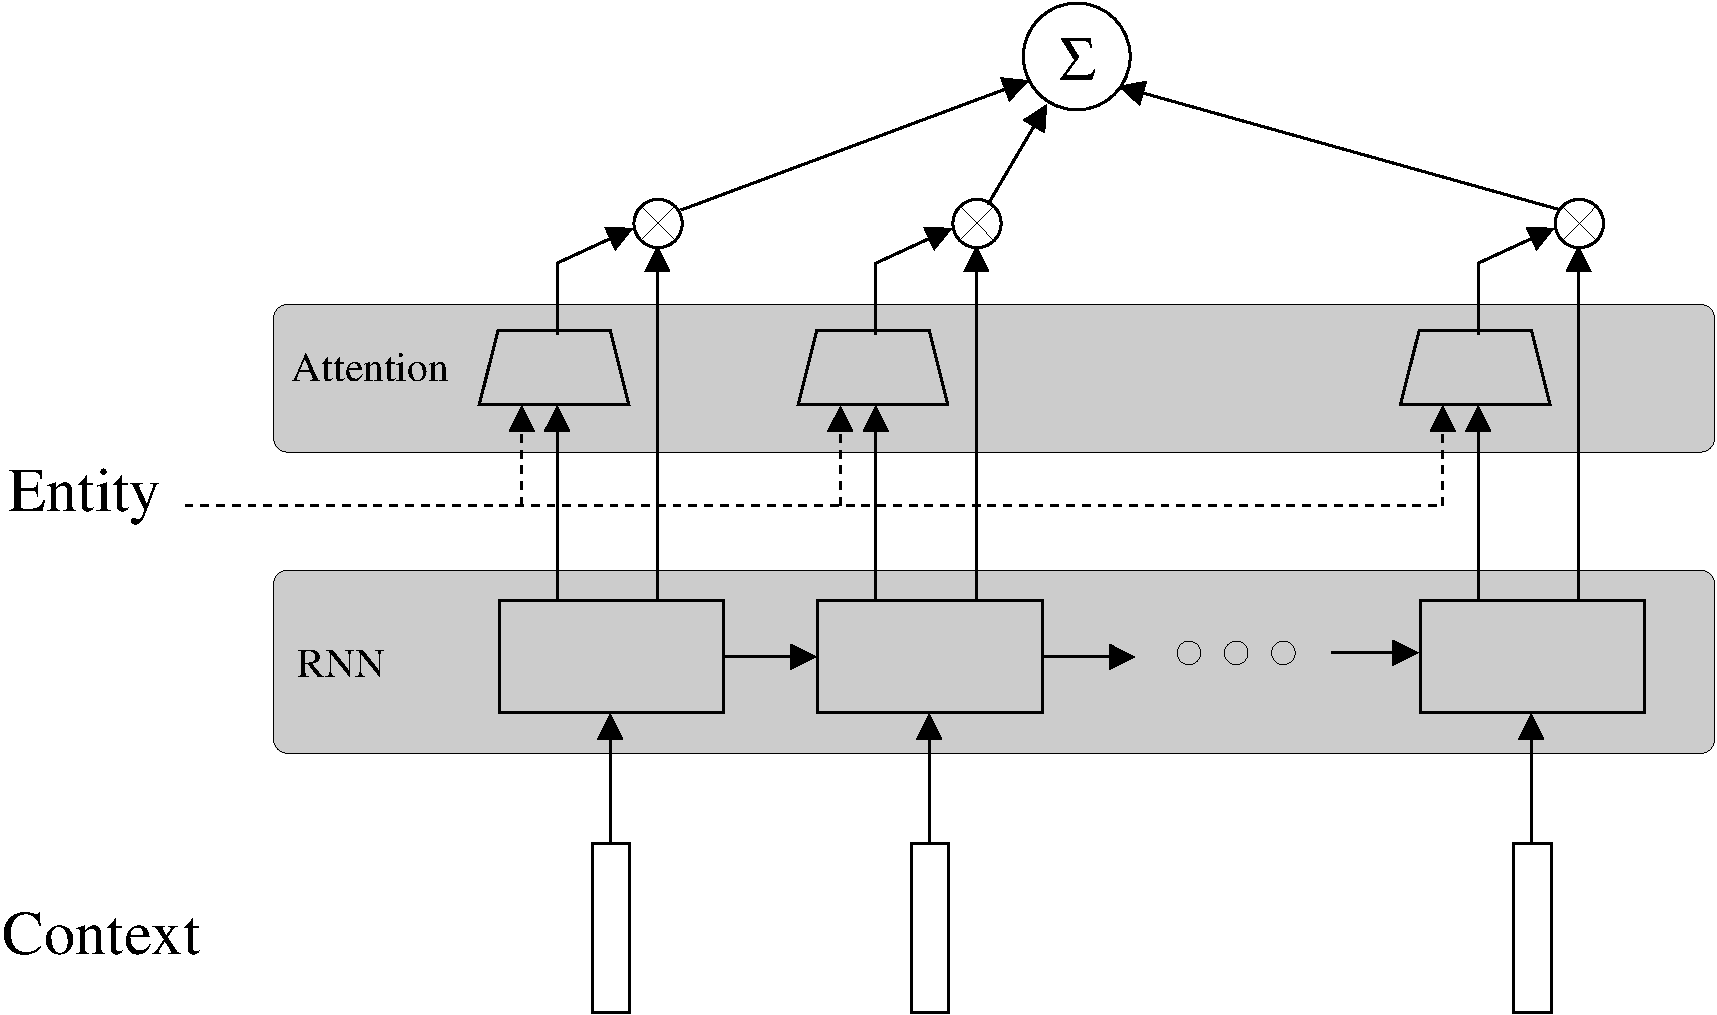
\includegraphics[scale=0.25]{diagrams/RNN_ATTN.pdf}
	\label{fig:arnn}
\end{figure}	

Our Attentional RNN component is based on a general RNN unit fitted with an attention mechanism. The mechanics of the Attentional RNN component are depicted in Figure \ref{fig:arnn}. 
	
Equation \ref{eq1} represents the general semantics of an RNN unit. An RNN reads a sequence of vectors $\{v_t\}$ and maintains a hidden state vector $\{h_t\}$. At each step a new hidden state is computed based on the previous hidden state and the next input vector by a function $f$ parametrized by $\Theta_1$. The output at each step is computed from the hidden state using a function $g$ parametrized by $\Theta_2$. This allows the RNN to 'remember' important signals while scanning the context and to recognize signals spanning multiple words.

\begin{equation}
\label{eq1}
\begin{aligned}
& h_t=f_{\Theta_1}(h_{t-1}, v_t) \\
& o_t=g_{\Theta_2}(h_t)
\end{aligned}
\end{equation}

In out implementation we have used a standard GRU unit \cite{cho2014learning}, however any RNN can be a drop-in replacement. While an RNN unit can be used as-is in our model by feeding the last output vector $o_t$ directly into the classifier network, we have implemented an attention mechanism that allows the model to be aware of the candidate entity it is evaluating when computing an output. Equation \ref{eq2} details the equations governing the attention model.

\begin{equation}
\label{eq2}
\begin{aligned}
& a_t \in \mathbb{R}; a_t=r_{\Theta_3}(o_t, v_{candidate}) \\
& a'_t  = \frac{1}{\sum_{i=1}^{t} \exp\{a_i\}} \exp \{a_t\} \\
& o_{attn}=\sum_{i=1}^{t} a'_t o_t
\end{aligned}
\end{equation}

The main component in equation \ref{eq2} is the function $r$, parametrized by $\Theta_3$, which computes an attention value at each step using $v_{candidate}$, the candidate entity embedding, as a control signal. We use the softmax function to normalize the attention values such that $\sum_{i=1}^{t} a'_i = 1$ and compute the final output $o_{attn}$ as a weighted sum of all the output vectors of the RNN. This allows the attention mechanism to decide on the importance of different context parts when examining a specific candidate. We parametrize our attention function $r$ as a single layer NN as shown in equation \ref{eq3} where $A, B$ are the layer weights and $b$ is a bias term.

\begin{equation}
\label{eq3}
r_{\Theta_3}(o_t, v_{candidate}) = Ao_t + Bv_{candidate} + b \\
\end{equation}


\subsection{Training initial word and entity embeddings}

Training our model implicitly trains its dictionaries of both word and entity embedding by error back-propagation. However, as will be shown in section \ref{experiments}, we have found using pre-trained embeddings to \hl{significantly improve model performance/greatly reduce training time(??)}. To this end we have devised a Skip Gram with Negative Sampling (SGNS) \cite{mikolov2013distributed} based training procedure that simultaneously trains both word and entity vectors in the same embedded space.

We use the word2vecf library\footnote{Available at https://bitbucket.org/yoavgo/word2vecf} by Levy and Goldberg \shortcite{levy2014dependency} that is adapted from word2vec code and allows to train on a dataset made of $(word,context)$ pairs rather then a textual corpus in string format, as is done in the original word2vec. We exploit this to redefine $context$ as a context entity rather then a contextual word. 

We do this by considering each page in Wikipedia to represent a unique entity, enumerated by the $pageid$ identifier in Wikipedia database and having a textual description (the page itself). For each word $\{word_i\}$ in the page we add the pair $(word_i,pageid)$ to our dataset. We however limit our vocabularies by ignoring both rare words that appear less then $20$ times and entities that have less then $20$ words in their description.
	
As shown by Levy and Goldberg \shortcite{levy2014neural} training embeddings on this dataset using SGNS produces word and entity embedding that implicitly factorize the word-entity co-occurrence PPMI matrix. This matrix is closely related to the TFIDF word-entity matrix used by Gabrilovich and Markovitch \shortcite{gabrilovich2007computing} in Explicit Semantic Analysis and found to be useful in a wide array of NLP tasks. 

For our experiments we trained embeddings of length 300 for 10 iterations over the dataset. We used default values for all other parameters in word2vec.

\hl{-needs developing-}

\hl{-show results of the analogies experiment we did indicating semantic structure for the WORD vectors-}

\section{\label{sec:w}Creating a Web-Fragment based NED Dataset}
We introduce a new large-scale NED dataset of web-fragments crawled from the web. Our dataset is derived from the Wikilinks dataset originally collected by Singh at el. \shortcite{singh12:wiki-links} for a cross-document co-reference task. cross-document co-reference entails clustering mentions referring to the same entity across a set of documents without consulting a predefined knowledge base of entities, and is many-a-time regarded as a downstream task for knowledge base population (KBP). Wikilinks was constructed by crawling the web and collecting hyperlinks linking to Wikipedia and the web context they appear in. The anchor texts act as mentions and the link targets in Wikipedia act as ground-truths. Wikilinks contains 40 million mentions covering 3 million entities and collected from over 10 million web pages.

Wikilinks can be seen as a large-scale, naturally-occurring and crowd-sourced dataset where thousands of human annotators provide ground-truths for mentions of interest. Its web sourcing entails every kind of noise expected from automatically gathered web content, including many faulty, misleading and peculiar ground truth labels on the one hand, and on the other hand noisy, malformed and incoherent textual context for mentions. While noise in crowd-sourced data is arguably a necessary trade-off for quantity, we believe the contextual noise in particular represents an interesting test-case that supplements existing standard datasets such as CoNLL \cite{hoffart2011robust}, ACE and Wiki \cite{ratinov2011local} as these are all sourced from mostly coherent and well formed text such as news articles and Wikipedia pages. Wikilinks emphasizes utilizing strong and adaptive local disambiguation techniques, and marginalizes the utility of coherency based global approaches.

The original dataset exists in a number of formats, and we have chosen a version with only short local contexts\footnote{Available at http://www.iesl.cs.umass.edu/data/wiki-links} since it renders the size of the dataset a manageable 5Gb of compressed data (compared to 180Gb for the full texts). Following are the filtering and preprocessing steps used to create a NED evaluation dataset from Wikilinks:

\begin{itemize} 
	\item we resolved ground-truth links using a $7/4/2016$ dump of the Wikipedia database\footnote{Recent Wikipedia dumps are found at https://dumps.wikimedia.org/}. The same dump was consistently used throughout this research. We used the $page$ and $redirect$ tables for resolution and kept the database $pageid$ column as a unique identifier for Wikipedia pages (entities). To reduce loss of unresolved mentions due to malformed URLs we compared page names using a case-insensitive and normalized\footnote{Normalization was done using the unidecode python library} title matching. We discarded mentions where the ground-truth could not be resolved, resulting in retention of $97\%$ of the mentions.
	\item We collected all pairs of mention $m$ and entity $e$ appearing in the dataset and computed the following two statistics: how many times $m$ refers to $e$: $\#\{e|m\}$ and the conditional probability of $e$ given $m$: $p(e|m)=\#\{e|m\}/\sum_{e'}\#\{e'|m\}$. Examining these distributions revealed many mentions belong to two extremes: either they had very little ambiguity or had a number of candidate entities each appearing very few times. We have deemed the former to be unambiguous and not-interesting, and the latter to be suspected as noise with high probability. We therefore designed a procedure to filter both this cases: We retained only mentions for whom at least two ground-truth entities have $\#\{e|m\}\ge 10$ and $p(e|m)\ge0.1$. 
	\item Finally, We randomly permuted the order of mentions within the data and split it into train, evaluation and test set. We split the data $90\% / 10\% / 10\%$ respectively. Since websites might include duplicate or closely related content we did not assign mentions into splits on an individual basis but rather collected all origin domains and assigned each domain along with all mentions collected from it into a split collectively.
\end{itemize}

This procedure aggressively filtered the dataset and we were left with $2.6M$ training, $300K$ test and $300K$ evaluation samples. We believe that doing so filters uninteresting cases while emitting a dataset that is large-scale yet manageable in size for research purposes. We note that we have considered filtering $(m,e)$ pairs where $\#\{e|m\}\le 3$ since these are suspected as additional noise however decided against this procedure as it might filter out long-tail entities, a case which was deemed interesting by the community.

\section{Evaluation} \label{experiments}

In this section we describe the setup used when evaluating our model and present evaluation results for two datasets. We evaluate the effect of initializing word and entity embeddings on our model as well.

\subsection{Wikilinks}

Prior to evaluating our method on the Wikilinks dataset we have collected the following statistics from the Wikilinks training set: $P(e)$ is the prior probability of seeing entity $e$ in the training set and $P(e|m)$ is the probability of seeing entity $e$ as a ground-truth for mention $m$. 

When evaluating a NED system it is required to use some method for generating candidate entities first. We use a simple method where given mention $m$, we considered all candidates for whom $P(e|m)>0$ as candidates. This simple method gives $97\%$ ground-truth recall on the test set. 
We used GRUs as our RNN unit and used fixed size left and right contexts, using a 20 word window to each side of the mention. In cases were the context was shorter than the fixed size, we padded it with a special $PAD$ symbol. Further, we filtered out stop words according to NLTK's stop-word list.
The optimization of the model was carried out using standard back propagation and an AdaGrad optimizer \cite{duchi2011adaptive}. We allowed the error to propagate through all parts of the network and fine tune all trainable parameters, including the word and entity embeddings themselves. A single epoch with $2.6M$ mentions and $k=5$ for corrupt example generation was used for training the model taking half a day using a 20-core CPU machine.

We have used the following methods as base line on the Wikilink dataset:

\begin{itemize} 
	\item  \textbf{Yamada et al.} \shortcite{Yamada2016} have created a state-of-the-art NED system for jointly mapping entities and words onto the same vector space via the skip-gram model and using these for disambiguation. As Wikilinks has only one mention per fragment we use only the local features described by Yamada at el.
	
	\item \textbf{Cheng et al.} \shortcite{Cheng2013} addressed the Disambiguation to Wikipedia, or the "Wikificaiton" task, with a combination of local and global approaches. Mentions are disambiguated locally by generating a ranked list of candidates for each mention using the GLOW Wikification system proposed by Ratinov et al. \shortcite{Ratinov2011}. We compare our results to the ranking step of the algorithm, were a linear Ranking SVM is trained over a set of local and global features to return the list of candidates sorted by their likelihood.
	
	\item We include Most Probable Sense (MPS) as a baseline. This baseline picks the entity with the highest $P(e|m)$ as the correct mention. This simple baseline is notoriously known to give competitive results in many NED datasets 
\end{itemize}

\subsection{CoNLL}
CoNLL is an evaluation corpus created by Hoffart et al. \shortcite{hoffart2011robust} commonly used for benchmarking NED solutions \cite{Globerson2016,Hachey2013,Yamada2016,Pershina2015}. CoNLL was composed by manually annotating Reuters newswire articles from 1996. It contains $1393$ documents from a period of $12$ days split into train, development and test sets. Following previous works we have only evaluated our method on non-NIL mentions. For candidate generation we used the publicly available candidate dataset by Pershina at el. \shortcite{Pershina2015} with over $99\%$ gold sense recall.

CoNLL has a training set with $18505$ non-NIL mentions, which preliminary experiments showed is not sufficient to train our model on. We therefore resorted to a more complex training method where we first trained our model on a large corpus of mentions derived from Wikipedia cross references and then fine tuned the resulting model on CoNLL training set. To derive the Wikipedia training corpus we have extracted all cross-reference links from Wikipedia along with their context, resulting in over $80$ million training examples. Due to constrained resources we set $k=1$ for corrupt example generation and trained $1$ epoch, which took around $4$ days to train. The resulting model was then fine-tuned on CoNLL training set, where corrupt examples were produced by considering all possible candidates for each mention.

We have also found that using traditional statistical and string based features along with our model further improves its performance. We therefor used a setting similar to Yamada et al. \shortcite{yamada2016joint} where a Gradient Boosted Regression Tree was fitted with our models prediction score as a feature along with $7$ other statistical and string based features. The statistical features are prior probability $P(e)$ and conditional probability $P(e|m)$ as described above, along with a feature counting the number of candidates generated for the mention and a feature giving the maximum conditional probability of the entity for all mentions in the document. For string similarity features we used the edit distance between the mention and the entity title in Wikipedia, a feature indicating weather the mention is a prefix or postfix of the entity Wikipedia title and a feature indicating weather the Wikipedia entity title is a prefix or postfix of the mention. Following Yamada we used sklearn's GradientBoostingClassifier implementation \cite{pedregosa2011scikit} with a deviance loss and set the learning rate, number of estimator and maximum depth of a tree to $0.02$, $10000$ and $4$, respectively. 

As a baseline we took the standard Most Probable Sense (MPS) prediction, which corresponds to the $\arg\max_{e\in{{E}}}{P(e|m)}$, where $E$ is the group of all candidate entities.
We also compare to the following papers - Lazic et al. \shortcite{Lazic2015}, Francis-Landau et al. \shortcite{Francis-Landau2016}, He et al. \shortcite{He2013}, Hoffart et al. \shortcite{hoffart2011robust} and Chisholm et al. \shortcite{Chisholm2015} ,as they are all strong local approaches and a good source for comparison.
	
\subsection{Results}

\begin{table}[h]
	\begin{center}
		\begin{tabular}{|c| p{1.5cm}|}
			\hline \multicolumn{2}{|c|}{Wikilinks test set} \\
			\hline \bf Model & \bf Micro     accuracy  \\ \hline
			ARNN  &  \bf64.8\\
			GBRT: Base + ARNN features & \bf 66.8 \\
			Yamada et al.(partial) & $59.8$ ** \\
			Cheng et al. & * \\ 
			Baseline (MPS) & $55.9$ \\
			\hline
		\end{tabular}
	\end{center}
	\caption{\label{tab:b} Evaluation on Web-Fragment data (Wikilinks)}
\end{table}

The micro and macro accuracy scores on CoNLL test-b are displayed in table \ref{tab:a}. 

	
\begin{table}[h]
	\begin{center}
		\begin{tabular}{|p{3.5cm}| p{1.5cm} p{1.5cm}|}
			\hline \multicolumn{3}{|c|}{CoNLL test-b} \\
			\hline Model & Micro     accuracy & Macro     accuracy \\ \hline
			\bf ARNN  & \bf $87.3$ & \bf $88.6$ \\
			\bf GBRT: Base + ARNN features & \bf $86.9$ & \bf $89.1$ \\
			Yamada et al. (partial) & $90.9$ & $92.4$ \\
			Lazic et al. & $86.4$ & - \\
			Francis-Landau et al. & $85.5$ & - \\
			He et al. & 84.82 & $83.37$ \\	
			Hoffart et al. & $79.57$ & $80.71$ \\
			Chisholm et al. & $88.7$ & - \\			
			Baseline (MPS) & $77$ & $77$ \\
			\hline
		\end{tabular}
	\end{center}
	\caption{\label{tab:a} Evaluation on CoNLL. Bold font denotes the models offered in this study}
\end{table}


add insights regarding the results and comparison 
\subsection{Model sensitivity}

\toin{Where is ARNN w/o init but with attention?}

\hl{Noam: this should be extended} elaborate on: \newline
!! ESA embedding initialization \newline
!! attention vs. no attention\newline

\begin{table}[h]
\begin{center}
	\begin{tabular}{|c| p{1.5cm}|}
		\hline \multicolumn{2}{|c|}{Wikilinks test set} \\
		\hline \bf Model & \bf Micro     accuracy  \\ \hline
		ARNN w/o ESA init. & $61$ \\
		ARNN w/ ESA init. w/o Attention & $64.1$ \\
		ARNN w/ ESA \& Attention & $64.8$ \\ 
		\hline
	\end{tabular}
\end{center}
\caption{\label{tab:c} ARNN Model sensetivity}
\end{table}

\section{Conclusions}

\bibliographystyle{acl2016}
\bibliography{_our_submission,_noam_bib}

\end{document}
